\appendix

% make sure you have a blank slide in case you accidentally go past your conclusion
\begin{frame}[plain]
\end{frame}


% these slides are to help answer potential questions and generally arent shown
% unless needed or there is extra time
\begin{frame}[plain]{Logistic Regression}
Logistic regression,
\begin{figure}
\centering
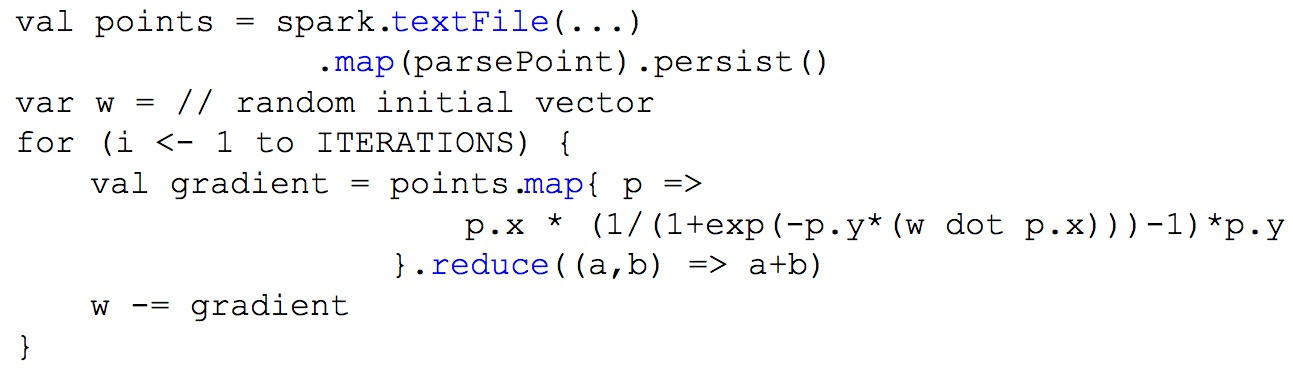
\includegraphics[width=0.9\linewidth]{figures/logistic-regression.jpg}
\end{figure}
\begin{itemize}
  \item \texttt{points} is a persistent RDD produced by \texttt{map} on text
  file
  \item repeatedly run \texttt{map} and \texttt{reduce} to compute gradient at
  each step by summing function of the current w.
  \item keeping \texttt{points} in memory across iterations yields 20x speedup.
\end{itemize}
\end{frame}

\begin{frame}[plain]{Word Count}
\begin{figure}
\centering
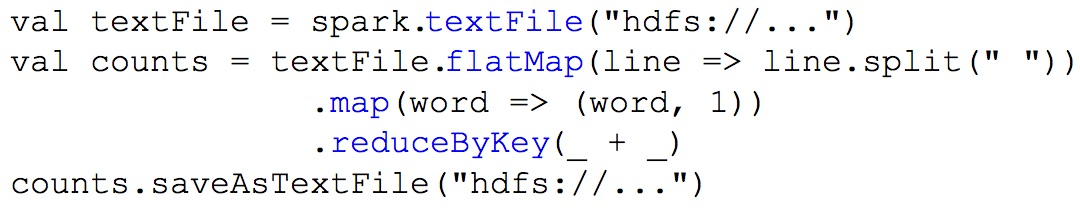
\includegraphics[width=0.9\linewidth]{figures/word-count.jpg}
\end{figure}
\end{frame}

\begin{frame}[plain]{Performance Tuning}
Problems,
\begin{itemize}
  \item Too few partitions
  \item Large per-key \texttt{groupBy()}
  \item Shipped all data across the cluster 
\end{itemize}

Guidelines
\begin{itemize}
  \item Ensure enough partitions (often 100 - 10000), mostly based on task
  execution time at least 100ms (upper bound), at least ~2x number of cores in
  cluster (lower bound)
  \item Minimize memory consumption while sorting and large keys in groupBys
  \item Minimize amount of data shuffled  
\end{itemize}

Resolution
\begin{itemize}
  \item Increase \texttt{spark.executor.memory}
  \item Increase number of partitions
  \item Re-evaluate program structure   
\end{itemize}
\end{frame}

\begin{frame}[plain]{Example 2 Optimization}
\begin{figure}
\centering
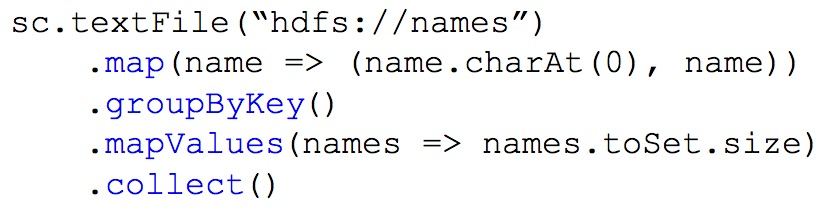
\includegraphics[width=0.9\linewidth]{figures/example2.jpg}
\end{figure}

\begin{figure}
\centering
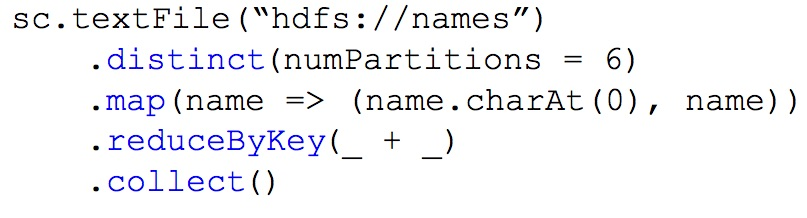
\includegraphics[width=0.9\linewidth]{figures/example2-optimized.jpg}
\end{figure}
\end{frame}

